\graphicspath{ {images/} }
\chapter{Proposed System}
\hspace{5mm} The proposed System has the main component as securing BYOD devices i.e. MDM server which handle android based smart phones so those mobiles will be used inside the orgnization efficently and securely. Since the system is used for the purpose of giving internet privileges to employees’ devices, only basic operations from the MDM server side can be performed (like device lock, passcode policy, etc.). The system allows the user to enroll to the MDM server from both within the network (company WiFi) and also outside (using Cellular). When the user enrolls his/her device to the system via the private network, the device is given a session that can be used to access the internet.  


\section{Analysis/Framework/Algorithm}
\hspace{5mm} Adroid devices(smartphone,tablet)are preferable with os android version 4.0 onwards.
The basic requirement for device is ,that device should not be rooted.That is downloading from other servers should be enable.From android device interface user connects to MDM server through openn ssl connection by exchanging certificate which embbeded with android user file.
\section{Details of Hardware and Software}
\subsection{Software Requirements} 

\begin{itemize}
    \item OS
    \item Framework
    \item Server
    \item Database
\end{itemize}

\subsection{Hardware Requirements} 
\begin{itemize}
    \item Processor
    \item RAM
    \item ROM
    \item GPU
\end{itemize}

\section{Design Details}
\begin{figure}[h!]
\begin{center}
\scalebox{0.60}{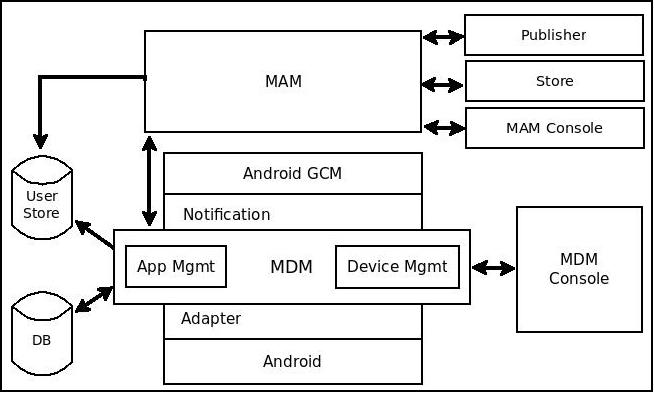
\includegraphics{system.jpeg}}
\end{center}
\caption {The Proposed System/System Architecture}
\label{vmb2}
\vspace{0mm}
\end{figure}

\par 
\begin{itemize}

    \item When the device connects to the private network, it checks with the router if it has a session. If so, then the device already has internet access in this network, else it will be redirected to the EMM server.
    \item The MDM server will check if the device is enrolled in the server.
    \begin{enumerate}
        \item If the device is already registered in the system, then it will direct the user to the WiFi Login page where the user would have to enter the LDAP credentials to get a new session.
        \item If not, it will be directed to the appropriate EMM page. In the case of Android, it will be directed to the MDM Agent download page whereas for iOS, it will be directed to the EMM registration page.
        \end{enumerate}
    \item Upon successfully enrolling the device to the EMM server, the server will automatically create a new session for the device.
\end{itemize}
\hspace{5mm} the system uses local massaging and Google Cloud Messaging(GCM).Carbon server API from WSO2 uses massaging service to send massgaes to user email id.Detail procedure about GCM is discuss in results.

\subsection{Detailed Design}
\hspace{5mm}In this section you need to put diagram/figures related to detailed design like UML diagrams. Also give small description about every diagram.(Must take suggestion from guide)  
\\
\begin{figure}[h!]
\begin{center}
\scalebox{0.50}{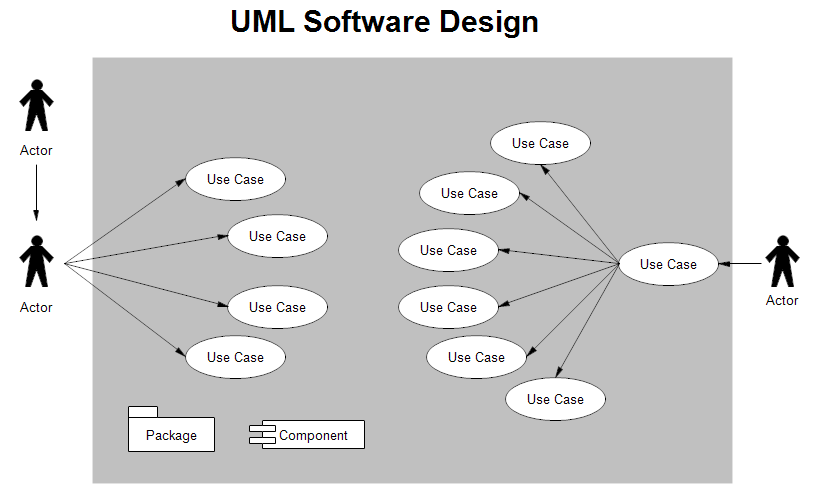
\includegraphics{images/usecase.png}}
\end{center}
\caption {use case}
\label{vmb2}
\vspace{0mm}
\end{figure}

\hspace{5mm}Small description about above diagram.

\begin{figure}[h!]
\begin{center}
\scalebox{1.00}{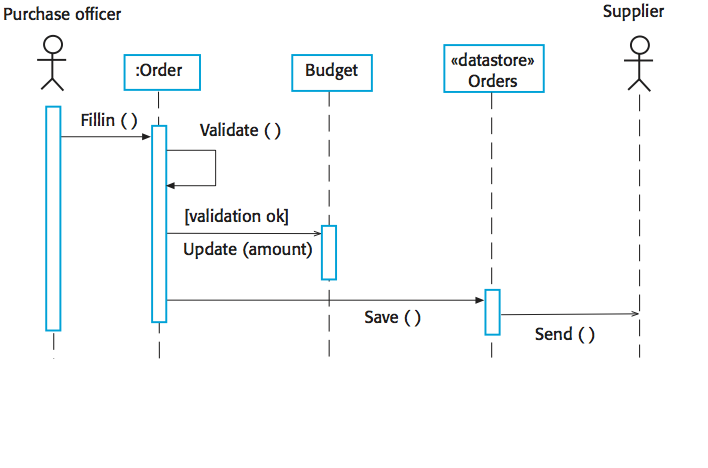
\includegraphics{images/sequence.png}}
\end{center}
\caption {Sequence Diagram}
\label{vmb2}
\vspace{0mm}
\end{figure}

\hspace{5mm}Small description about above diagram.

\section{Methodology/Procedures(your approach to solve the problem)} 
List to list all methodologies that you found during literature survey. Explain all algorithms that will be use in your project.

\hspace{5mm}In this section all algorithms or any other implementation procedure need to explain with proper flow.
\par describe every procedure or algorithm with necessary diagram.
\par also explain different technology or languages you used for implementation/Deployment.

\begin{table}[h!]
  \begin{center}
    \caption{Your first table.}
    \label{tab:table1}
    \begin{tabular}{l|c|r} % <-- Alignments: 1st column left, 2nd middle and 3rd right, with vertical lines in between
      \textbf{Value 1} & \textbf{Value 2} & \textbf{Value 3}\\
      $\alpha$ & $\beta$ & $\gamma$ \\
      \hline
      1 & 1110.1 & a\\
      \hline
      2 & 10.1 & b\\
      3 & 23.113231 & c\\
    \end{tabular}
  \end{center}
\end{table}

\begin{table}[ht]
\caption{Nonlinear Model Results} % title of Table
\centering % used for centering table
\begin{tabular}{c c c c} % centered columns (4 columns)
\hline\hline %inserts double horizontal lines
Case & Method\#1 & Method\#2 & Method\#3 \\ [0.5ex] % inserts table
%heading
\hline % inserts single horizontal line
1 & 50 & 837 & 970 \\ % inserting body of the table
2 & 47 & 877 & 230 \\
3 & 31 & 25 & 415 \\
4 & 35 & 144 & 2356 \\
5 & 45 & 300 & 556 \\ [1ex] % [1ex] adds vertical space
\hline %inserts single line
\end{tabular}
\label{table:nonlin} % is used to refer this table in the text
\end{table}

\subsection{Procedures} 
Some mathematical formulae
\\
\[ x^n + y^n = z^n \]
\\
Multiple integrals.
\\
$\iint_V \mu(u,v) \,du\,dv$$
\\
\\
Sums and products
\\
Sum \sum_{n=1}^{\infty} 2^{-n} = 1$ inside text
\\
$$\sum_{n=1}^{\infty} 2^{-n} = 1$$
\\
\\
\[
    \binom{n}{k} = \frac{n!}{k!(n-k)!}
\]
\\
\\
When displaying fractions in-line, for example \(\frac{3x}{2}\) 
you can set a different display style: 
\( \displaystyle \frac{3x}{2} \).
 
This is also true the other way around
 
\[ f(x)=\frac{P(x)}{Q(x)} \ \ \textrm{and} 
\ \ f(x)=\textstyle\frac{P(x)}{Q(x)} \]






\pagebreak